\subsection{无限族代数的张量积}

设 A 是一个交换环， \((\mathrm{E}_{i})_{i\in\mathbb{I}}\) 是任意一族（含单位元的）A-代数。对 I 的每个有限子集 J，令 \(E_{J}\) 表示张量积 \(\bigotimes_{i\in J}E_{i}\) ，其中诸代数 \(E_{i}\) 的指标 \(i\in J\) ；令 \(e_{i}\) 表示 \(E_{i}\) 的单位元，令 \(e_{J}=\bigotimes_{i\in J}e_{i}\) 表示 \(E_{J}\) 的单位元；令 \(f_{J,i}\) 表示典范同态 \(E_{i}\to E_{J}\) （对 \(i\in J\) ）（第 2 号, 命题 5）。若 J, \(J'\) 是 I 的两个有限子集且 \(J\subset J'\) ，则典范地导出一个同态 \(f_{J'J}:E_{J}\to E_{J'}\) （第 2 号, 命题 5），其条件是 \(f_{J'J}\circ f_{J,i}=f_{J',i}\) 对所有 \(i\in J\) 成立。此外， \(f_{J'J}\) 的唯一性蕴含：若 J, \(J',J''\) 是 I 的三个有限子集且 \(J\subset J'\subset J''\) ，则 \(f_{J''J}=f_{J''J'}\circ f_{J'J}\) 。换言之， \((\mathrm{E}_{\mathrm{J}},f_{\mathrm{J}'\mathrm{J}})\) 是一个 A-代数的正向系统，其指标集是 I 的有限子集构成的右有向集 \(\mathfrak{F}(\mathbf{I})\) 。

定义 5. 正向系统 \((\mathbf{E}_{\mathbf{J}}, f_{\mathbf{J}^{\prime}\mathbf{J}})\) 的正向极限 E 称为 A-代数族 \((\mathbf{E}_i)_{i \in \mathbf{I}}\) 的张量积 .

若 I 有限，则 E 等同于 \(\bigotimes_{i\in I}E_i\) 。滥用记号，即使 I 无限，E 也记作 \(\bigotimes_{i\in I}E_i\) 。

对每个有限子集 \(J\) （取自 \(I\) ），令 \(f_{J}\) 表示典范同态 \(\bigotimes_{i \in J} E_{i} \to \bigotimes_{i \in I} E_{i}\) （写作 \(f_{i}\) 而非 \(f_{(i)}\) ）；若 \(e\) 是 \(\bigotimes_{i \in I} E_{i}\) 的单位元，则 \(f_{J}(e_{J}) = e\) 对所有 \(J \in \mathfrak{F}(I)\) 成立。显然，若所有代数 \(E_{i}\) 都是交换的，则 \(\bigotimes_{i \in I} E_{i}\) 也是交换的 .

命题 8. (i) 诸同态 \(f_{i} \colon \mathbf{E}_{i} \to \mathbf{E} = \bigotimes_{k \in \mathbf{I}} \mathbf{E}_{k}\) 满足：对两个指标 \(i, j\) ，当 \(i \neq j, f_{i}(x_{i})\) 与 \(f_{j}(x_{j})\) 在 \(\mathbf{E}\) 中对所有 \(x_{i} \in \mathbf{E}_{i}\) 和 \(x_{j} \in \mathbf{E}_{j}\) 交换；进而 \(\mathbf{E}\) 由诸子代数 \(f_{i}(\mathbf{E}_{i})\) 的并生成 .

\begin{enumerate}
\def\labelenumi{(\roman{enumi})}
\setcounter{enumi}{1}
\item
  设 \(\mathbf{F}\) 是一个 A-代数，且对所有 \(i \in \mathbf{I}\) ，设 \(u_i: \mathbf{E}_i \to \mathbf{F}\) 是 A-代数同态，使得对 \(i \neq j\) ， \(u_i(x_i)\) 与 \(u_j(x_j)\) 在 \(\mathbf{F}\) 中对所有 \(x_i \in \mathbf{E}_i\) 和 \(x_j \in \mathbf{E}_j\) 交换。则存在且仅存在一个 A-代数同态 \(u: \mathbf{E} \to \mathbf{F}\) 使得 \(u_i = u \circ f_i\) 对所有 \(i \in \mathbf{I}\) 成立 .
\item
  由于对 I 的每一个有限子集 J， \(f_{i} = f_{J} \circ f_{J,i}\) ，(i) 中的第一个断言由第 2 号, 命题 5 得出（取包含 i 和 j 的 J）；第二个断言同样由第 2 号, 命题 5 得出，并考虑到 E 是诸 \(f_{J}(E_{J})\) 当 J 遍历 \(\mathfrak{F}(I)\) 时的并 .
\item
  对每个有限子集 \(\mathbf{J}\) （含于 \(\mathbf{I}\) ），由第 2 号, 命题 5 可知，存在唯一的同态 \(u_{\mathbf{J}}: \mathrm{E}_{\mathbf{J}} \to \mathrm{F}\) 使得 \(u_{\mathbf{J}} \circ f_{\mathbf{J},i} = u_{i}\) 对所有 \(i \in J\) 成立；由这一唯一性立即得出，对 \(J \subset J'\) ， \(u_J = u_{J'} \circ f_{J'J}\) ；换言之，诸 \(u_J\) 构成一个同态的正向系统。设 \(u = \varinjlim u_J: E \to F\) ；则按定义， \(u_J = u \circ f_J\) 对 \(J\) （ \(I\) 的每个有限子集）成立，特别地， \(u_i = u \circ f_i\) 对所有 \(i \in I\) 成立； \(u\) 的唯一性由这些关系及 \(f_i(E_i)\) 生成代数 \(E\) 这一事实得出 .
\end{enumerate}

推论. 设 \((\mathbf{E}_i)_{i\in \mathbf{I}}\) , \((\mathbf{E}_i')_{i\in \mathbf{I}}\) 是具有同一指标集的两族 A-代数，且对所有 \(i\in \mathbf{I}\) ，设 \(u_i\colon \mathbf{E}_i\to \mathbf{E}_i'\) 是代数同态。则存在且仅存在一个 A-代数同态 \(u\colon \bigotimes_{i\in \mathbf{I}}\mathbf{E}_i\to \bigotimes_{i\in \mathbf{I}}\mathbf{E}_i'\) 使得对所有 \(i\in \mathbf{I}\) ，图表

\pandocbounded{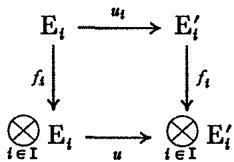
\includegraphics[keepaspectratio]{images/part003_14ac730d.jpg}}

是交换的，其中 \(f_{i}\) 和 \(f_{i}^{\prime}\) 表示典范同态。

只需将命题 8 应用于同态 \(f_{i}^{\prime} \circ u_{i}\) .

在命题 8 的推论中定义的同态 \(u\) 记作 \(\bigotimes_{i \in I} u_i\) 。若 \(J\) 是 \(I\) 的任意子集，则命题 8 可应用于典范同态族 \((f_i)_{i \in J}\) （诸 \(f_i: E_i \to \bigotimes_{i \in I} E_i = E\) ）；由此导出一个典范同态 \(E_J \to E\) ，它同样记作 \(f_J\) ，且当 \(J\) 有限时，它与上文中这样记的同态一致。

现在设 \((x_{i})_{i\in \mathbf{I}}\) 是 \(\prod_{i\in \mathbf{I}}\mathrm{E}_i\) 的一个元素，使得族 \((x_{i} - e_{i})_{i\in \mathbf{I}}\) 具有有限支撑 H。显然，若 J 和 \(J^{\prime}\) 是 I 的两个包含 H 的有限子集，则

\[
f _ {J} ((x _ {i}) _ {i \in J}) = f _ {J ^ {\prime}} ((x _ {i}) _ {i \in J ^ {\prime}}).
\]

 \(f_{\mathbf{J}}((x_i)_{i \in \mathbf{J}})\) （其中 \(\mathbf{J} \supset \mathbf{H}\) 遍历 \(\mathbf{I}\) 的有限子集）的公共值记为 \(\bigotimes_{i \in \mathbf{I}} x_i\) .

命题 9. 设 \((\mathbf{E}_i)_{i\in \mathbf{I}}\) 是一族 A-代数，且对每个 \(i\in \mathbf{I}\) ，设 \(B_{i}\) 是 \(\mathbf{E}_i\) 的一组基，使得单位元 \(e_i\) 属于 \(\overline{\mathbf{B}}_i\) 。设 \(\mathbf{B}\) 是形如 \(\bigotimes_{i\in \mathbf{I}}x_i\) 的元素组成的集合，其中 \((x_{i})\) 取遍 \(\prod_{i\in \mathbf{I}}\mathbf{B}_i\) 中使族 \((x_{i} - e_{i})\) 具有有限支撑的元素。则 \(\mathbf{B}\) 是代数 \(\bigotimes_{i\in \mathbf{I}}\mathbf{E}_i\) 的一组基，且这组基包含单位元 \(e\) .

对 I 的每个有限子集 J，设 \(B_{J}\) 是 \(E_{J} = \bigotimes_{i \in J} E_{i}\) 的基，即诸基 \(B_{i}\) （ \(i \in J\) ）的张量积（II, §3, 第 9 号）。由定义立即得出，B 是诸 \(f_{J}(B_{J})\) 当 J 遍历 \(\mathfrak{F}(I)\) 时的并，且 \(f_{J^{\prime}J}(B_{J}) \subset B_{J^{\prime}}\) 当 \(J \subset J^{\prime}\) 时成立；因此 \((B_{J})\) 是诸 \(E_{J}\) 的子集的一个正向系统，且 \(B = \varinjlim B_{J}\) ；结论由 II, §6, 第 2 号, 命题 5 的推论得出。

基 B 也称为诸基 \(B_{i}\) （ \(i \in I\) ）的张量积；当命题 9 的条件满足时，典范同态 \(f_{J}: E_{J} \to E = \bigotimes_{i \in I} E_{i}\) 对 I 的每个子集 J 都是单射，因为若 \(B_{J}\) 是 \(E_{J}\) 的基，即诸 \(B_{i}\) （ \(i \in J\) ）的张量积，则立即可以验证 \(f_{J}\) 在 \(B_{J}\) 上的限制是单射，且把 \(B_{J}\) 映到 B 的一个子集上。

